% title page

\begin{titlepage}
    \begin{center}
        \vspace{4cm}
        
        \rule{\textwidth}{1.2pt}
        
        \vspace{0.3cm}

        {\Huge \textbf{EJU PHY}}

        \vspace{0.3cm}

        {\LARGE A BRIEF SUMMARY}

        \vspace{0.3cm}

        {\Large \textit{version \version}}

        \rule{\textwidth}{1.2pt}

        \vspace{2cm}

        {\LARGE \textbf{PENG AO}}

        \vspace{0.5cm}
        {\Large \today}

        \vfill

        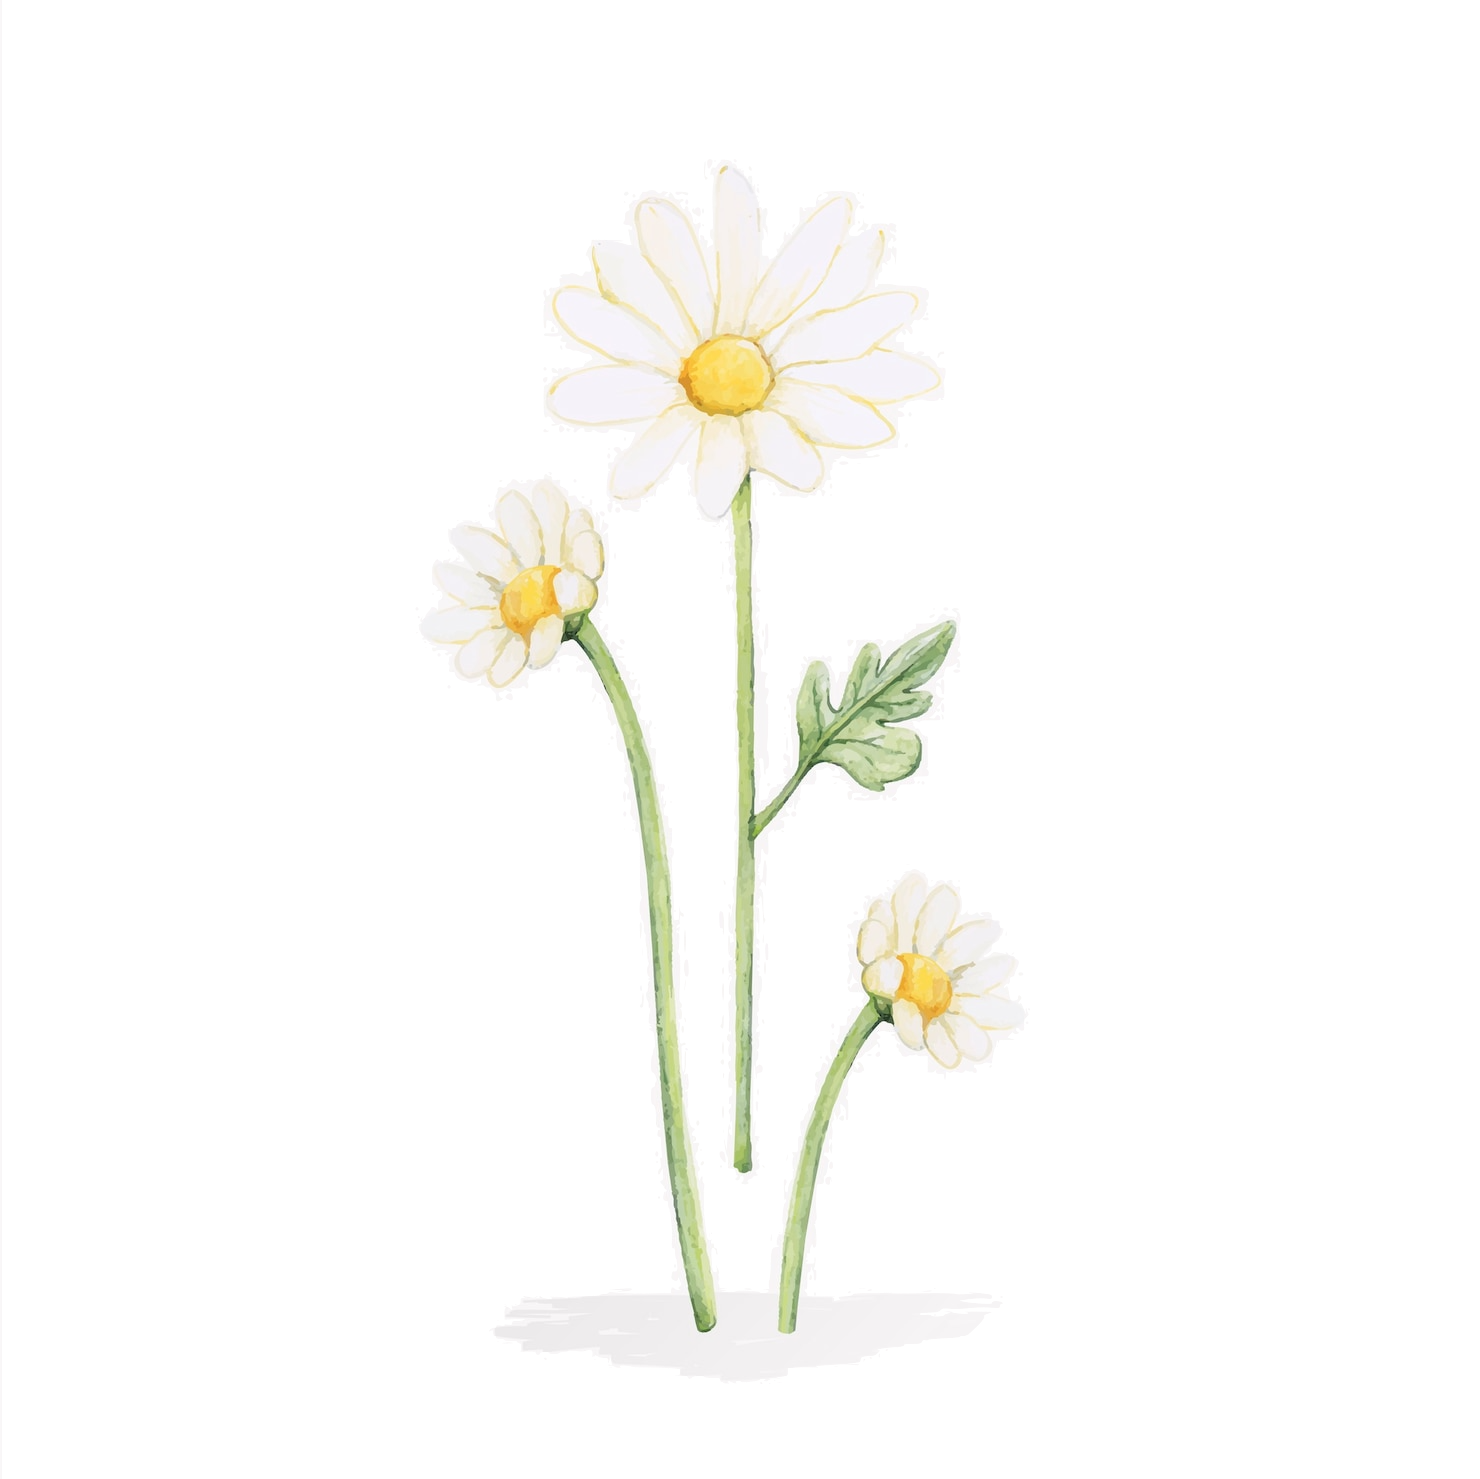
\includegraphics[width=0.382\textwidth]{autumn-cosmos.png}
    \end{center}
\end{titlepage}

% copyright

\clearpage
\begin{flushleft}
    \null

    \vfill
    
\includegraphics{by-nc-sa.png}

    This work is licensed under the Creative Commons Attribution-NonCommercial-ShareAlike 4.0 International License. To view a copy of this license, visit http://creativecommons.org/licenses/by-nc-sa/4.0/.

    \vspace{1em}
    You are free to:
    \begin{itemize}
        \item Share — copy and redistribute the material in any medium or format
        \item Adapt — remix, transform, and build upon the material
    \end{itemize}

    Under the following terms:
    \begin{itemize}
        \item Attribution — You must give appropriate credit, provide a link to the license, and indicate if changes were made. You may do so in any reasonable manner, but not in any way that suggests the licensor endorses you or your use.
        \item NonCommercial — You may not use the material for commercial purposes.
        \item ShareAlike — If you remix, transform, or build upon the material, you must distribute your contributions under the same license as the original.
    \end{itemize}
\end{flushleft}

% dedication

\clearpage
\begin{center}
    \null

    \vspace{0.382\textheight}
    \textit{\large
        To my gorgeous highschool life
        and meaningful college life.
    }
\end{center}

% preface

\clearpage
\chapter{前言}

\section*{自述}
本人PENG AO,来自于辽宁省沈阳市,大学本科四年级。目前就读于日本东京大学理学部情报科学科,即计算机科学专业。本文档脱胎于2019至2021年间个人授课时所整理的大纲,主要梳理了留学生统一考试理科物理的知识点,方便个人使用。

如今是2022年初春,正值本人即将迈入大学四年级之时。出于系统练习书写\LaTeX 文档,为今后学术报告、论文撰写做准备的目的,将此前的大纲进行了重新编辑。在书写过程中尽可能采取了清晰的书写结构,力争完全使用tikz绘图语言包来完成文档中的插图。

各章节内容参考了「わかりやすい高校物理の部屋」等网站和河合出版的《物理教室(四訂版)》等书籍,基于个人中学\footnote{东北育才外国语学校}时备考留学生统一考试时的所学所感加以补充。即便如此也难免有疏漏或是差错,欢迎在GitHub项目\footnote{https://github.com/PENG-AO/EJU-PHY}上开设Issue提出。

最后,对在教学过程中帮助我逐步做出优化调整的学生们以及编辑过程中辅助我校对的朋友们表示感谢。同时也希望能对有相关需求的读者起到一定的帮助作用。

\begin{center}
    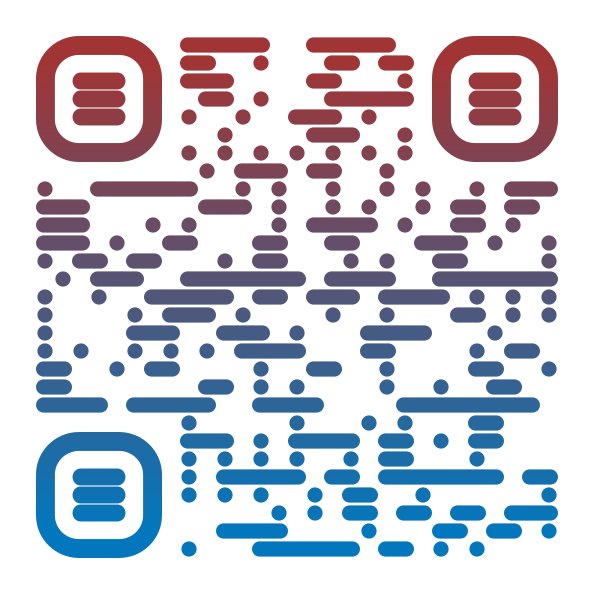
\includegraphics[width=0.16\textwidth]{repo-qrcode.png}
\end{center}

\begin{flushright}
    PENG AO\\
    2022-03-30 in Tokyo
\end{flushright}

\section*{历史}
\begin{itemize}
    \item \textit{version 1}:2019年手写版
    \item \textit{version 2}:2020年markdown电子版
    \item \textit{version 3}:2022年本文档
\end{itemize}

\section*{结构}
\begin{multicols}{2}
    \begin{itemize}
        \item 第一章:力学
        \item 第二章:热学
        \item 第三章:波动
        \item 第四章:电磁
        \item 第五章:原子
        \item 附录一:公式总结
        \item 附录二:延伸内容
        \item 附录三:历年考点
        \item 附录四:配图一览
        \item 附录五:推荐书目
    \end{itemize}
\end{multicols}
本书与留学生统一考试考纲顺序相同。正文部分只保留最必要的、无法进一步割舍的考点,附录中包含了一些相关数学知识的复习、个人自娱自乐\footnote{本人非物理相关专业,仅凭兴趣基于大学通识物理的知识试做推导,难免有所谬误}的定理推导过程、和一些其他信息的汇总。读者可以通过目录中的链接自由跳转阅读。

\section*{战绩}
本人考学时参加了2018年的两次留学生统一考试,其中6月份的在香港,11月份的在日本京都。凭借如下的留学生统一考试的成绩和97分\footnote{根据当年经验,97分的成绩在绝对数值上不具备十足的优势,但尚且够用}的托福成绩得到了东京大学理学部情报科学科、京都大学工学部情报学科、名古屋大学情报学部计算机科学科和东京工业大学的录取通知书。
\begin{center}
    \renewcommand\arraystretch{1.2}
    \begin{tabular}{c|cccc|c}
        \hline
        &日语&数学2&物理&化学&\\\hline
        2018.6&372(50)&192&95&85&744\\
        2018.11&374(45)&193&95&92&754\\
        \hline
    \end{tabular}
\end{center}

% toc

\clearpage
\renewcommand{\contentsname}{目录}
\tableofcontents
